\documentclass[12pt]{article}
\usepackage[english]{babel}
\usepackage{natbib}
\usepackage{url}
\usepackage[utf8x]{inputenc}
\usepackage{amsmath}
\usepackage{graphicx}
\graphicspath{{images/}}
\usepackage{parskip}
\usepackage{fancyhdr}
\usepackage{graphicx}
\usepackage{float}
\usepackage{vmargin}
\setmarginsrb{3 cm}{2.5 cm}{3 cm}{2.5 cm}{1 cm}{1.5 cm}{1 cm}{1.5 cm}

\title{Desarrollo de Aplicaciones Web \newline\newline Proyecto Final}          % Title
\author{A07104218}                                                              % Student ID
\date{November 29th, 2017}                                                      % Date

\makeatletter
\let\thetitle\@title
\let\theauthor\@author
\let\thedate\@date
\makeatother

\pagestyle{fancy}
\fancyhf{}
\rhead{\theauthor}
\lhead{\thetitle}
\cfoot{\thepage}

\begin{document}

%%%%%%%%%%%%%%%%%%%%%%%%%%%%%%%%%%%%%%%%%%%%%%%%%%%%%%%%%%%%%%%%%%%%%%%%%%%%%%%%%%%%%%%%%

\begin{titlepage}
    \centering
    \vspace*{0.5 cm}
    
\includegraphics[scale = 0.25]{logoITESM.png}\\[1.0 cm] % University Logo
    \textsc{\LARGE Instituto Tecnológico y de Estudios\newline\newline Superiores de Monterrey Campus\newline\newline Puebla}\\[2.0 cm] % University Name
    \textsc{\Large TC2026}\\[0.5 cm]                % Course Code
    \rule{\linewidth}{0.2 mm} \\[0.4 cm]
    { \huge \bfseries \thetitle}\\
    \rule{\linewidth}{0.2 mm} \\[1.5 cm]
    
%   \begin{minipage}{0.4\textwidth}
%       \begin{flushleft} \large
%           \emph{Submitted To:}\\
%           Ashish Kumar\\
%             Asst. Professor\\
%             Computer Science Department\\
%           \end{flushleft}
%           \end{minipage}~
%           \begin{minipage}{0.4\textwidth}
            
%           \begin{flushright} \large
%           \emph{Submitted By :} \\
%           Divjot Kaur\\
%             13103057\\
%             Group-G3\\
%             Semester\\
%       \end{flushright}
        
%   \end{minipage}\\[2 cm]
    
    
    \textbf{Alumno:} Salvador Orozco Villalever\\
    \textbf{Matrícula:} A07104218\\
    \textbf{Fecha:} 29 de noviembre de 2017\\
    \textbf{Profesor:} Dr. Adolfo Centeno Téllez\\
    
    
    
\end{titlepage}

%%%%%%%%%%%%%%%%%%%%%%%%%%%%%%%%%%%%%%%%%%%%%%%%%%%%%%%%%%%%%%%%%%%%%%%%%%%%%%%%%%%%%%%%%
\renewcommand{\contentsname}{Contenido}
\tableofcontents
\pagebreak

%%%%%%%%%%%%%%%%%%%%%%%%%%%%%%%%%%%%%%%%%%%%%%%%%%%%%%%%%%%%%%%%%%%%%%%%%%%%%%%%%%%%%%%%%

% \section{About this design}
% This is a simple report template with the UCT logo. Feel free to use/modify it to suit your needs. Variables that need to be altered have been commented to make modifications easier. For example if you need to change the university logo, look for the comment \texttt{\% University Logo} in this file and then make appropriate modifications in that line.

% A Table of Contents and a bibliography have also been implemented. To add entries to your bibliography, simply edit \texttt{biblist.bib} in the root folder and then use the \texttt{\textbackslash cite\{\ldots\}} command in \texttt{main.tex} \cite{bibtex}. The Table of Contents will be updated automatically.

% I hope that you find this template both visually appealing and useful. \\

% \hspace{1 cm}--- Linus

\section{Introducción}

El problema que se nos presentó para el proyecto final de la materia de Desarrollo de Aplicaciones Web consistía en elegir un tema en particular que nos interesara y construir entonces una aplicación web alrededor del mismo. La intención era poner en práctica lo visto en clase al respecto del desarrollo web a través del Google App Engine, una plataforma de este gigante de la tecnología que nos permite diseñar, desarrollar y montar aplicaciones web de manera fácil, rápida y gratuita. Aunque el desarrollo y las pruebas se hacen de forma local, con sólo unos comandos es posible desplegar la página web mandando el proyecto a la Google Cloud Platform, el lugar donde nuestro proyecto vivirá, de manera que la aplicación pueda ser visitada por cualquier persona.

\section{Descripción del problema}

El tema que yo elegí para mi proyecto fue el de la industria de venta y renta de bienes raíces. Elegí el tema anterior debido a que un familiar cercano es un profesional de esta industria en la Riviera Maya, un lugar en donde esto ha tenido un gran auge. La intención al desarrollar esta aplicación era permitir que cada usuario registrara y mostrara propiedades en esta aplicación web; para cada propiedad, debían almacenarse datos como el título, la dirección, la cantidad de habitaciones, el precio y una foto, entre otras cosas. Por otro lado, para que la aplicación fuera atractiva para los visitantes de la página, la interfaz gráfica debía ser lo suficientemente intuitiva y elegante.

\section{Definición de arquitectura}

En cuanto a la arquitectura, se trata de un esquema de tipo REST, el cual puede ser dividido en dos grandes secciones: el backend y el frontend. El siguiente esquema tomado de la documentación de Google muestra
cómo desde distintos clientes (web, android, iOS) podemos tener acceso a los endpoints que hemos ya desarrollado en el Google App Engine.

\begin{figure}[H]
\centering
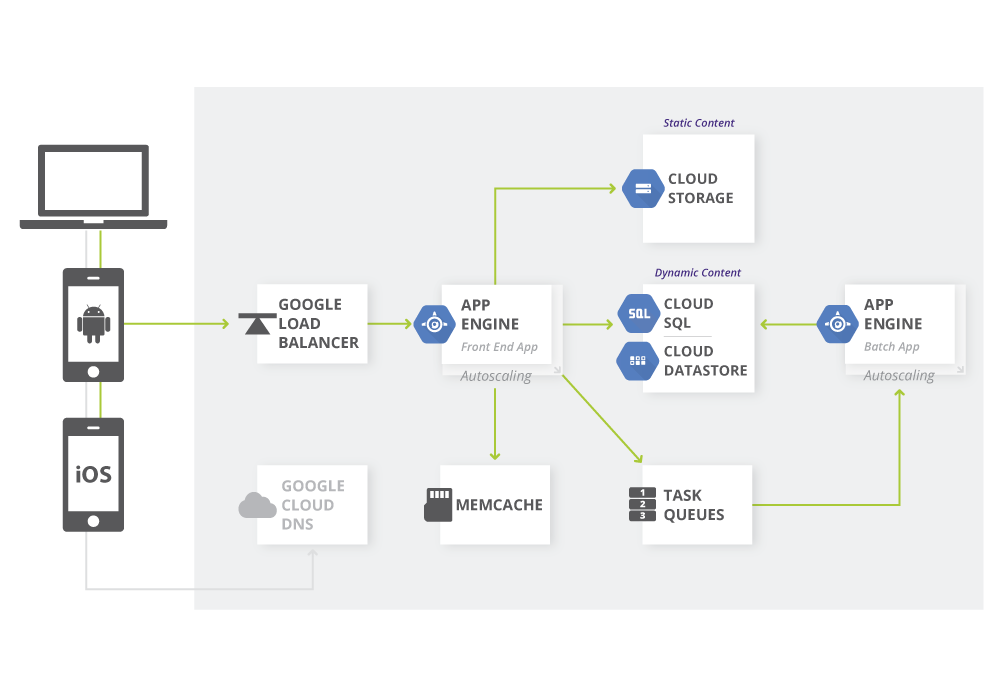
\includegraphics[width=0.75\textwidth]{01_WebApp_ArchDiagram.png}
\caption{Arquitectura de una aplicación en Google App Engine (GAE) tomado de [4]}
\end{figure} 

\subsection{Backend}

El Backend está construido sobre el Google Cloud SDK, específicamente utilizando la biblioteca cliente para Python en su versión 2.7. Esta sección cuenta con los siguientes elementos:

\begin{enumerate}
\item \textbf{Los modelos:} se trata de las entidades que son almacenadas en la base de datos proporcionada por el Google App Engine. Esta aplicación cuenta con las siguientes entidades:
  \begin{enumerate}
    \item Empresa: corresponde a una de las empresas que utilizarán esta aplicación.
    \item Usuario: corresponde a un colaborador de una de las empresas que utilizarán esta aplicación.
    \item Propiedad: corresponde a una casa, un departamento, un lote o un terreno que será registrado en la aplicación.
    \item Mensaje: corresponde a un texto corto que un visitante deja en la página web para pedir informes acerca de una propiedad en específico.
  \end{enumerate}
\item \textbf{Los mensajes:} se trata de los datos que el servidor escrito en Python recibe y responde según la solicitud que éste reciba. Distiguimos los siguientes mensajes:
    \begin{enumerate}
    \item Input: utilizado para crear una nueva instancia de una entidad
    \item List: utilizado para guardar todos los atributos de las instancias de una lista de entidade
    \item Update: utilizado para actualizar una instancia de una entidad
    \item Token: utilizado para demostrar que el usuario sí ha iniciado sesión
    \item TokenKey: utilizado para obtener los datos de una instancia específica de una entidad
    \item CodeMessage: utilizado para conocer el veredicto de una operación en el servidor
    \end{enumerate}
\item \textbf{Las APIs con token:} se trata de cuatro APIs para la administración de las entidades en la base de datos y para la seguridad de la aplicación. Esta aplicación cuenta con las siguientes APIs con token:
\begin{enumerate}
    \item Empresa: Delete, Get, Insert, List, Update
    \item Usuario: Delete, Get, Insert, List, Update, Login, Logout
    \item Propiedad: Delete, Get, Insert, List, Update
    \item Mensaje: Insert
\end{enumerate}
\item \textbf{La API pública:} se trata de una serie de controladores y rutas que nos permiten servir las vistas de la aplicación, vistas desde las cuales se hacen las llamadas a los controladores y al servidor
\item \textbf{El archivo de configuración de la aplicación:} se trata de un archivo que especifica cómo corresponden las URLs a los controladores de solicitudes y los archivos estáticos. Además, contiene información acerca del código de la aplicación.
\end{enumerate}

\subsection{Frontend}

El Frontend está basado en una plantilla adquirida en la tienda ThemeForest; el nombre de la plantilla es "Findeo Real Estate Template" y fue desarrollada con HTML, CSS y JavaScript. A través de una serie de archivos HTML, estilos en CSS y funciones en JavaScript es como se construyen las vistas y las animaciones y los efectos en éstas.

\section{Web services}

Cada entidad utilizada en esta aplicación web tiene su respectiva API escrita en Python con la cual es posible realizar las cuatro operaciones básicas de CRUD: create, retrieve, update y delete. Una vez que una API es desarrollada, ésta se convierte en un Google Cloud Endpoint lo que representa grandes beneficios como una arquitectura escalable que nos ofrece el rendimiento deseado. Además, se trata de APIs seguras pues utilizan el JSON Web Token para validar las llamadas; Google proporciona Auth0 y Firebase Authentication para ello. Por otro lado, a través de un proxy de servicio, se garantiza la seguridad y disponibilidad de la información en menos de un milisegundo por cada llamada. Finalmente, es posible desarrollar todo lo anterior en Python (el lenguaje que elegimos en esta ocasión) o Java con los frameworks abiertos de los Cloud Endpoints.

\section{Lenguaje de programación}

El lenguaje de programación utilizado para el desarrollo del servidor web es Python. Si bien era posible crearlo con otro lenguaje como Java, NodeJS, Ruby o Go, considero que Python es un excelente lenguaje debido a la agilidad de desarrollo que nos proporciona y a la gran cantidad de refefencias, ejemplos y recursos disponibles en la web. Además, al tratarse del lenguaje por excelencia en el área de Machine Learning, resultará muy práctico para implementar en un futuro el algoritmo KNN para recomendar propiedades similares a aquellas que el usuario visite. Para el cliente de Android, el lenguaje utilizado fue Java, pues se generaron clases a partir del código de Python.

\section{Base de datos}

La base de datos utilizada es la famosa NDB, una base de datos de tipo NoSQL con la característica de que es altamente escalable. Cuenta también con replicación automática para garantizar la disponibilidad y durabilidad de los datos. Además, soporta consultas de tipo SQL, índices, transacciones ACID, entre otras cosas. Utilizando la biblioteca de Google Datastore NDB para Python es que logré conectar esta aplicación web a esa base de datos.

\section{Tecnologías del cliente}

Entre las tecnologías utilizadas para el desarrollo de los clientes web y Android destacan las siguientes:

\begin{enumerate}
\item Python
\item Java
\item jQuery
\item HTML
\item CSS
\item XML
\item Google App Engine
\item Google Data Store
\item Google Blob Storage
\item JavaScript
\end{enumerate}

\section{Anexos}

\begin{figure}[H]
\centering
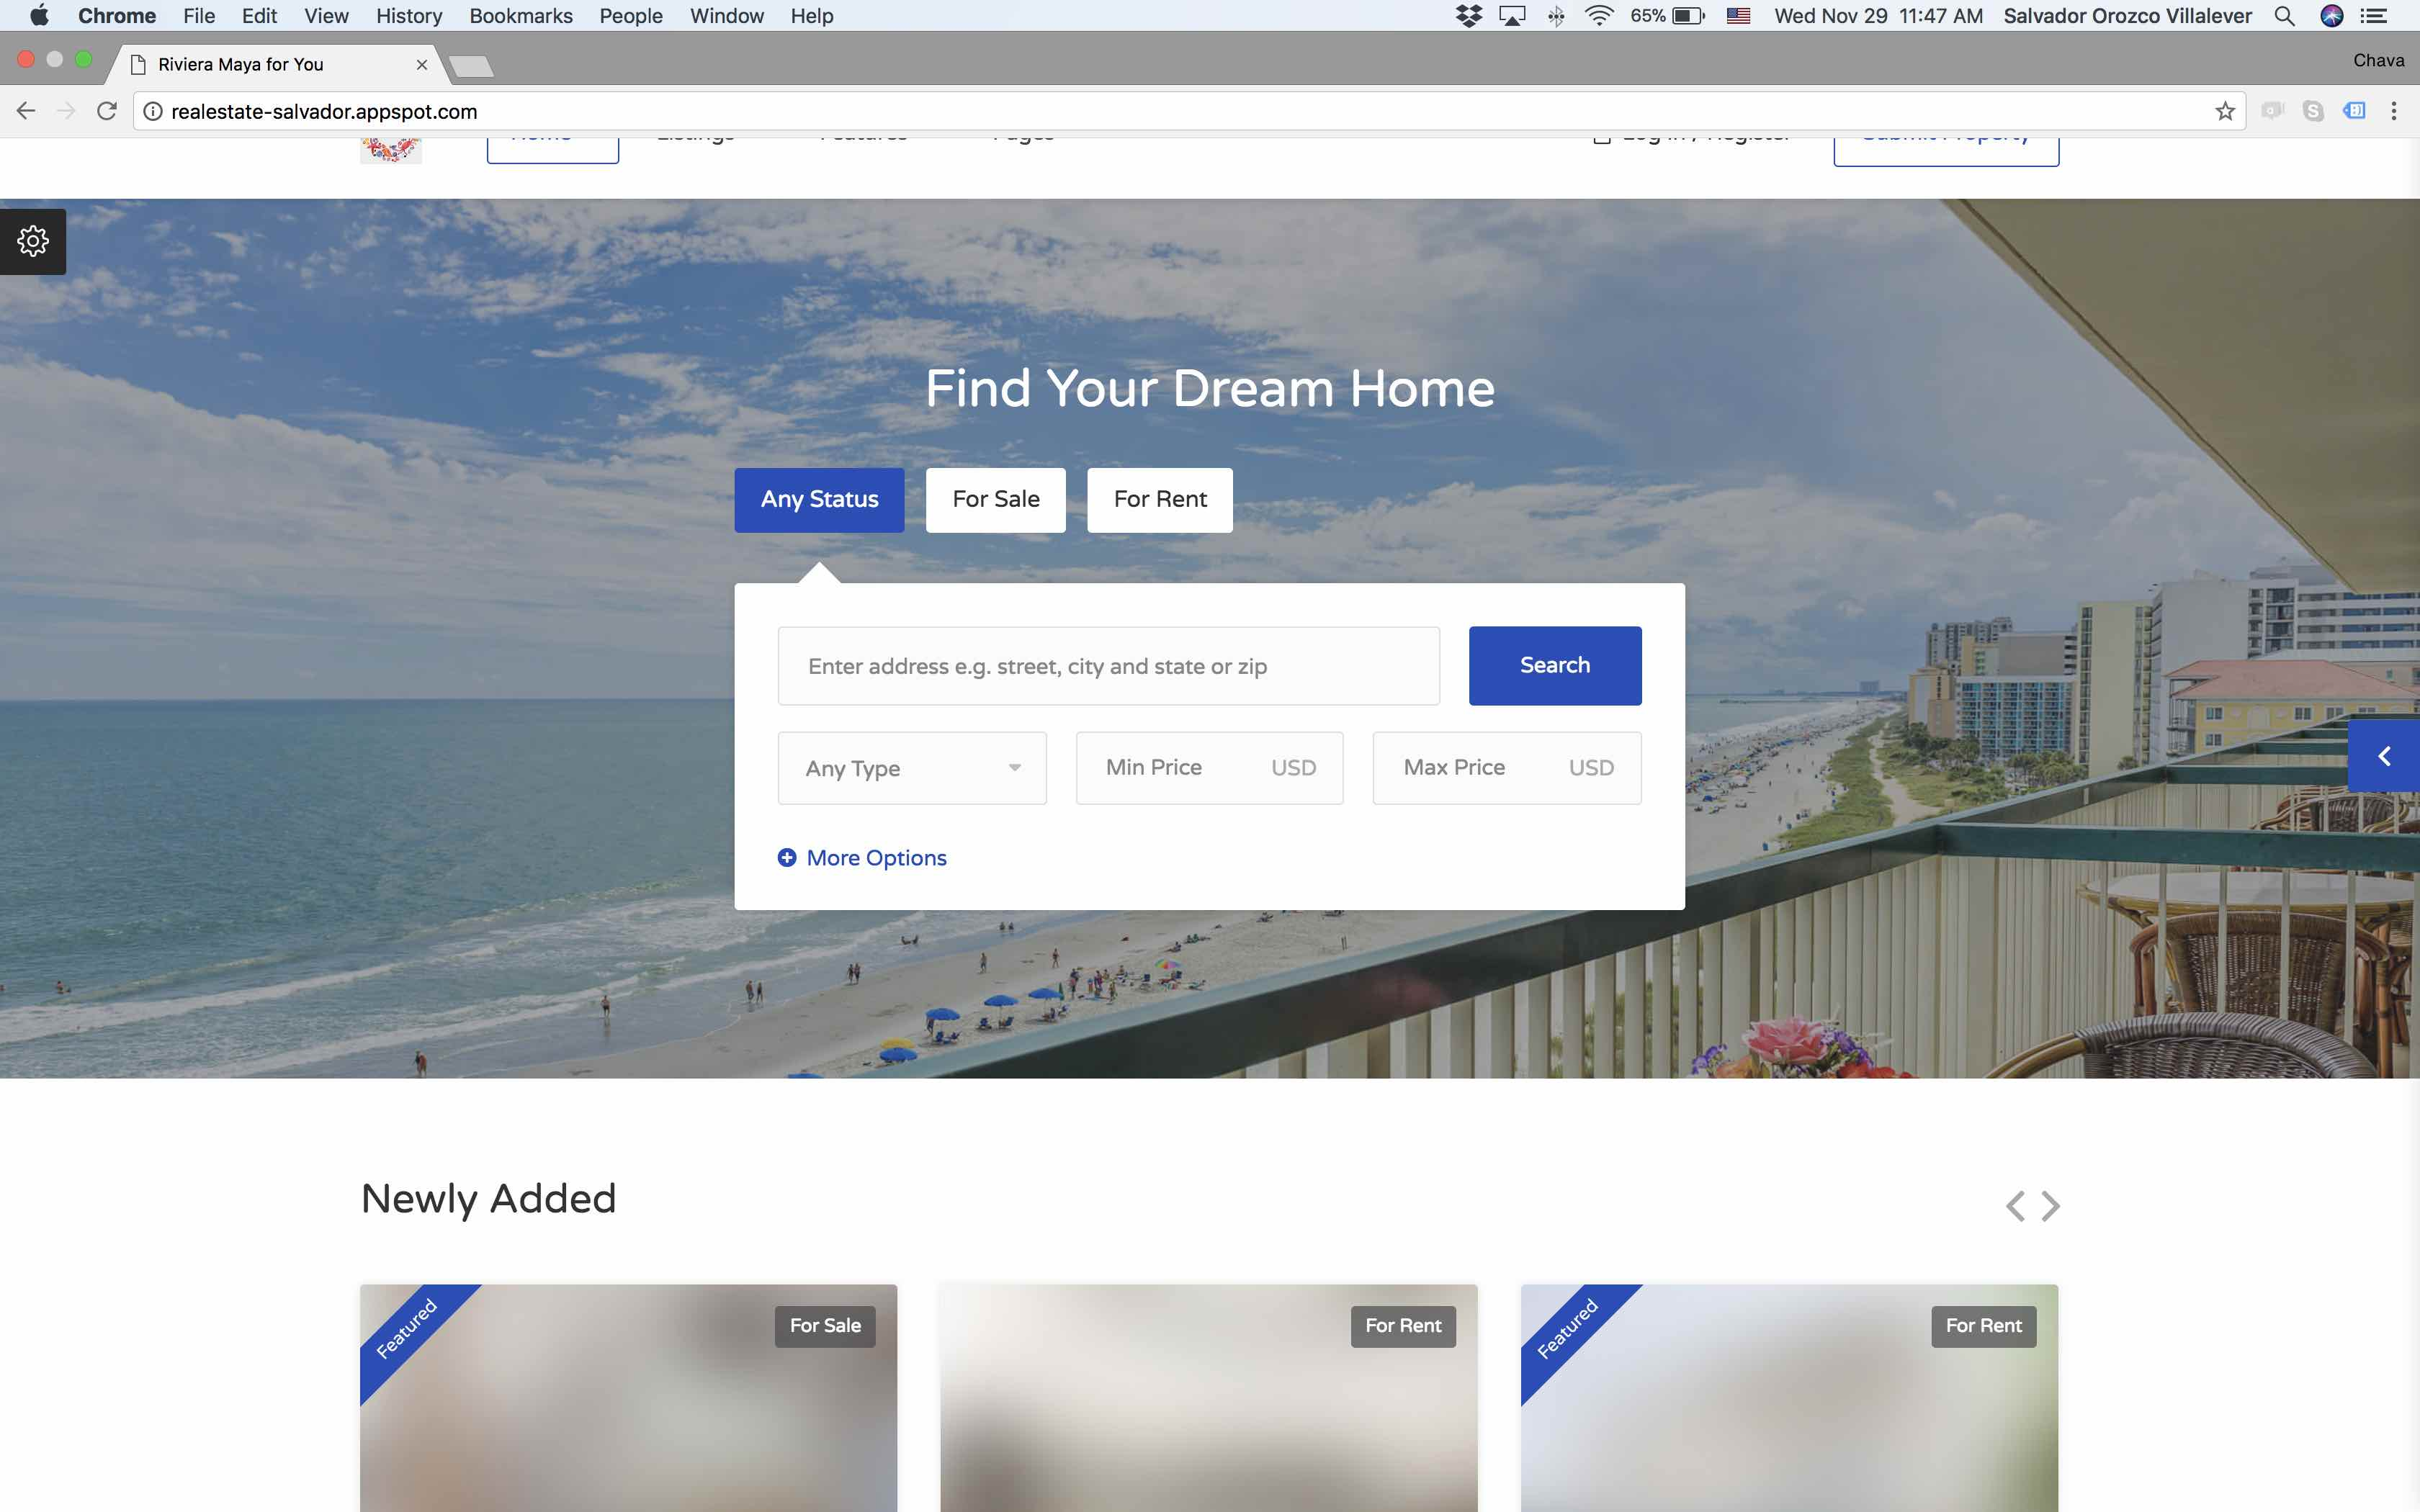
\includegraphics[width=0.75\textwidth]{img1.jpg}
\caption{}
\end{figure} 

\begin{figure}[H]
\centering
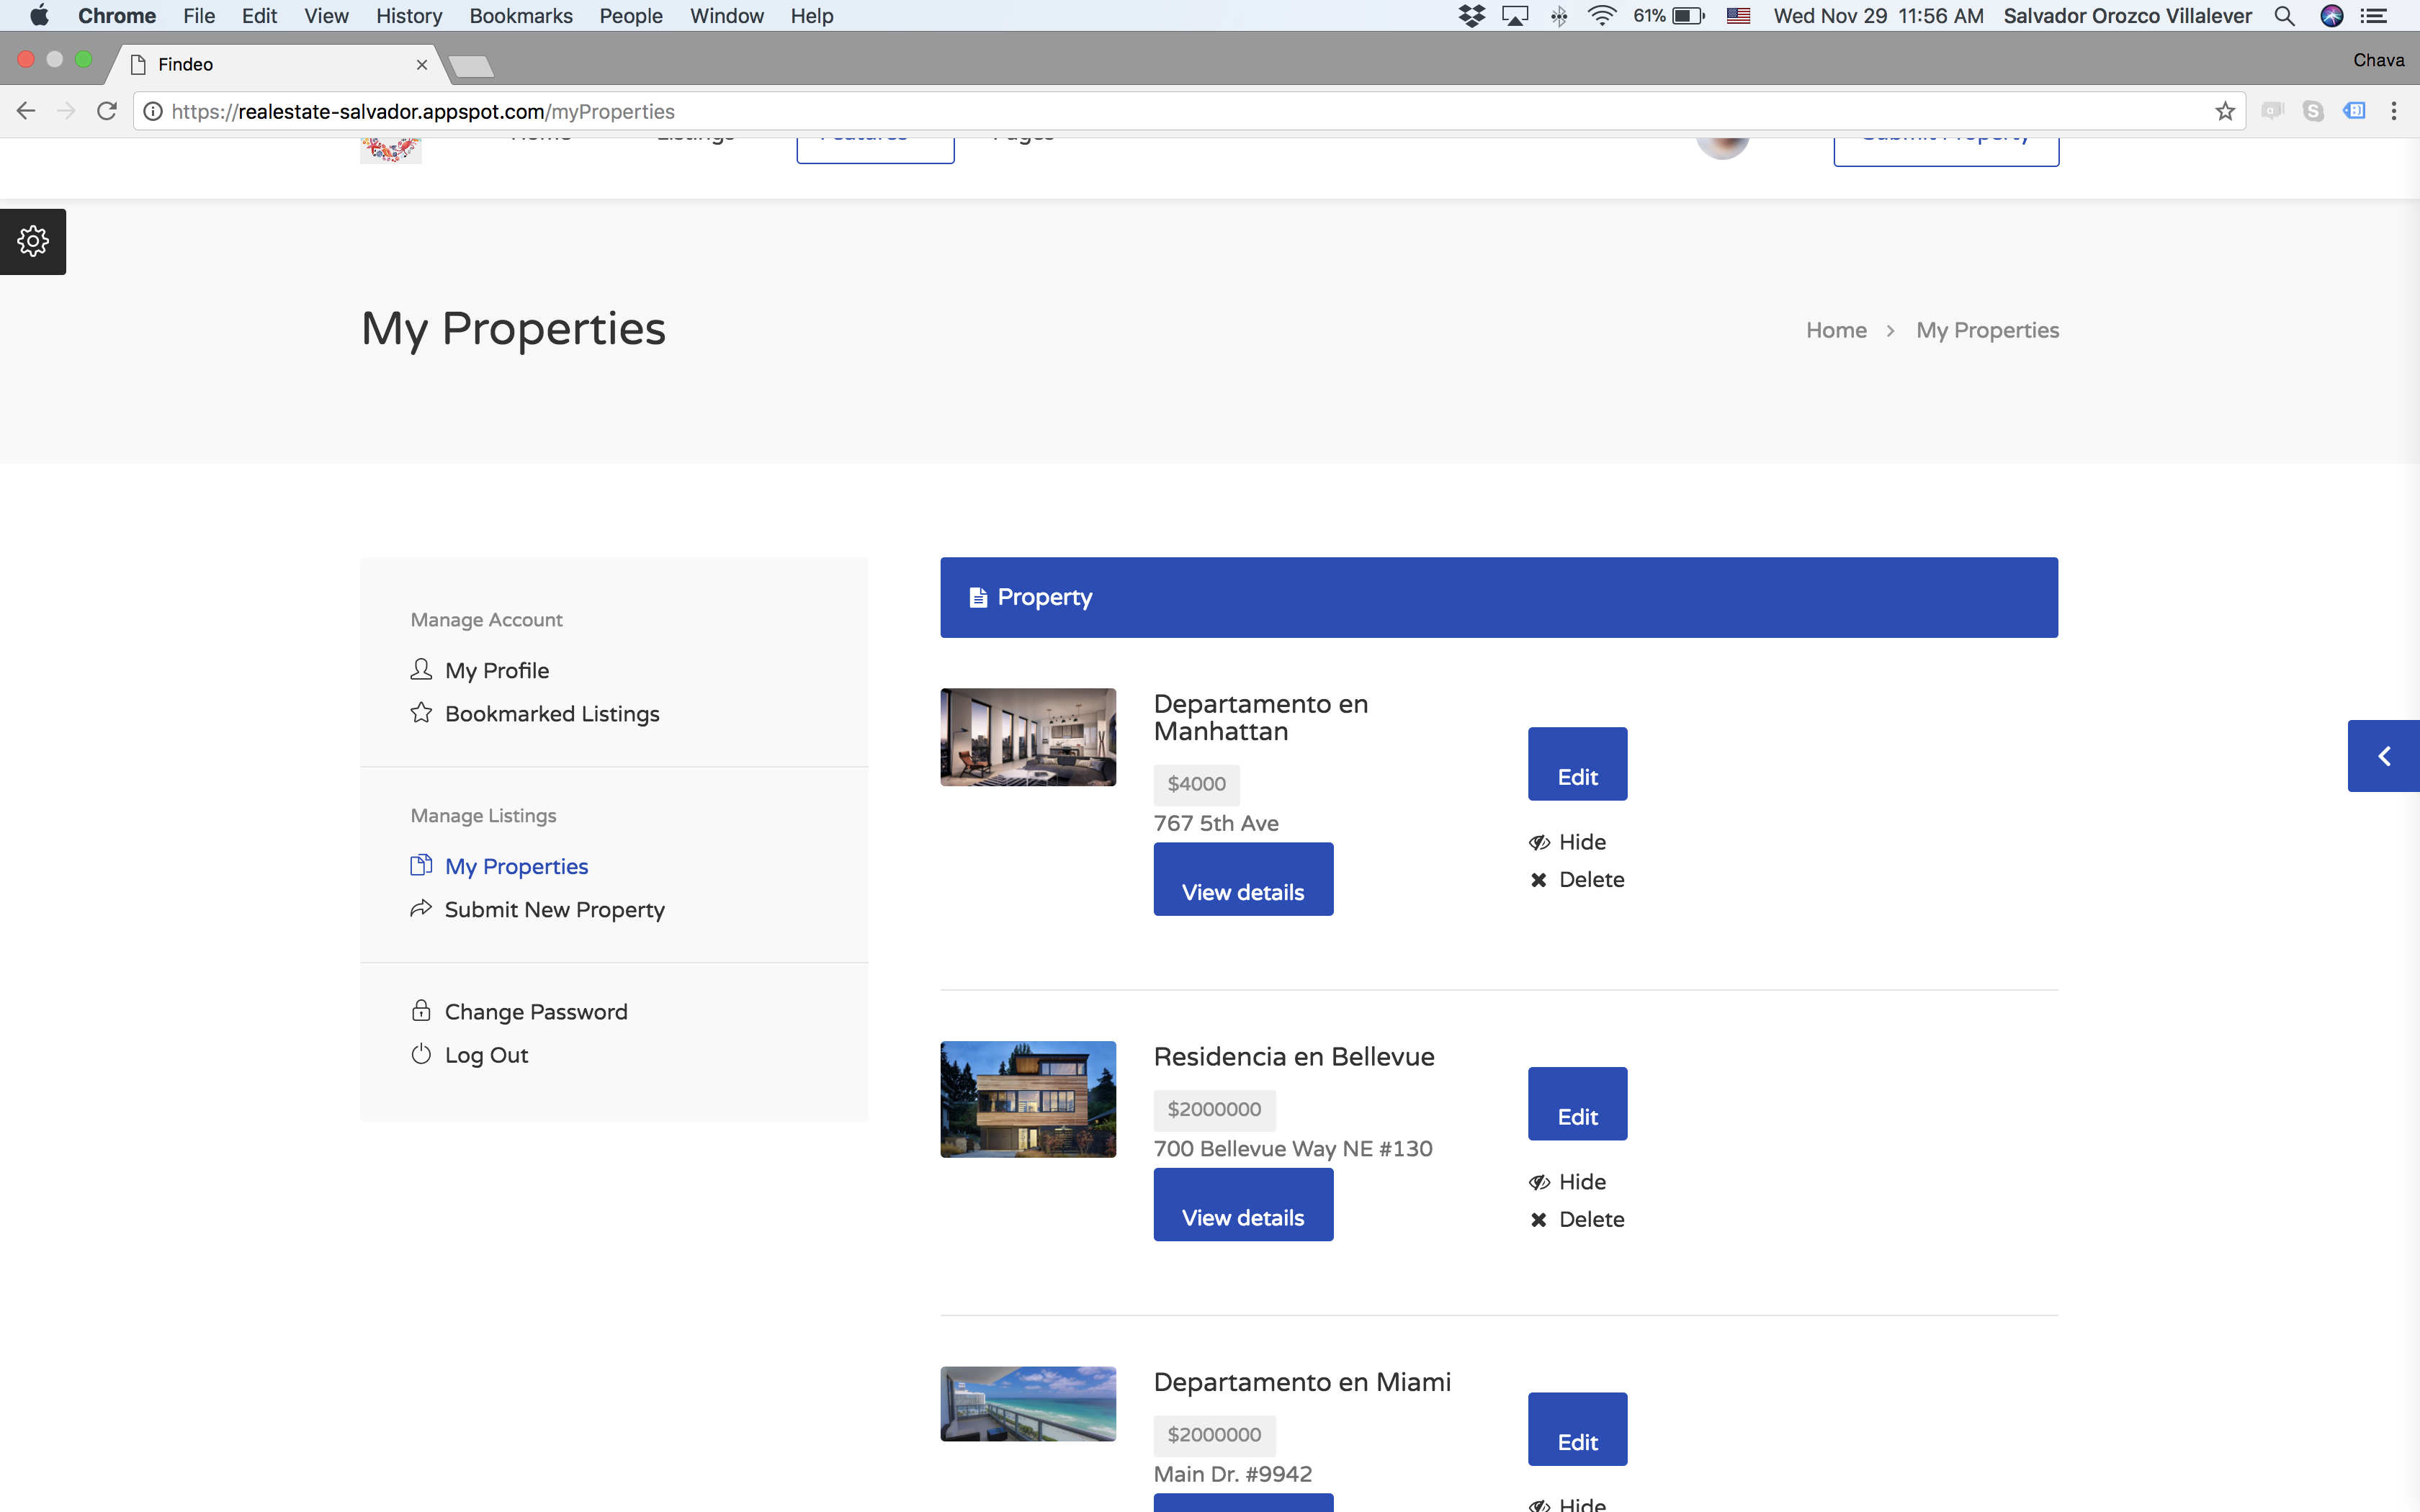
\includegraphics[width=0.75\textwidth]{img2.png}
\caption{}
\end{figure} 

\begin{figure}[H]
\centering
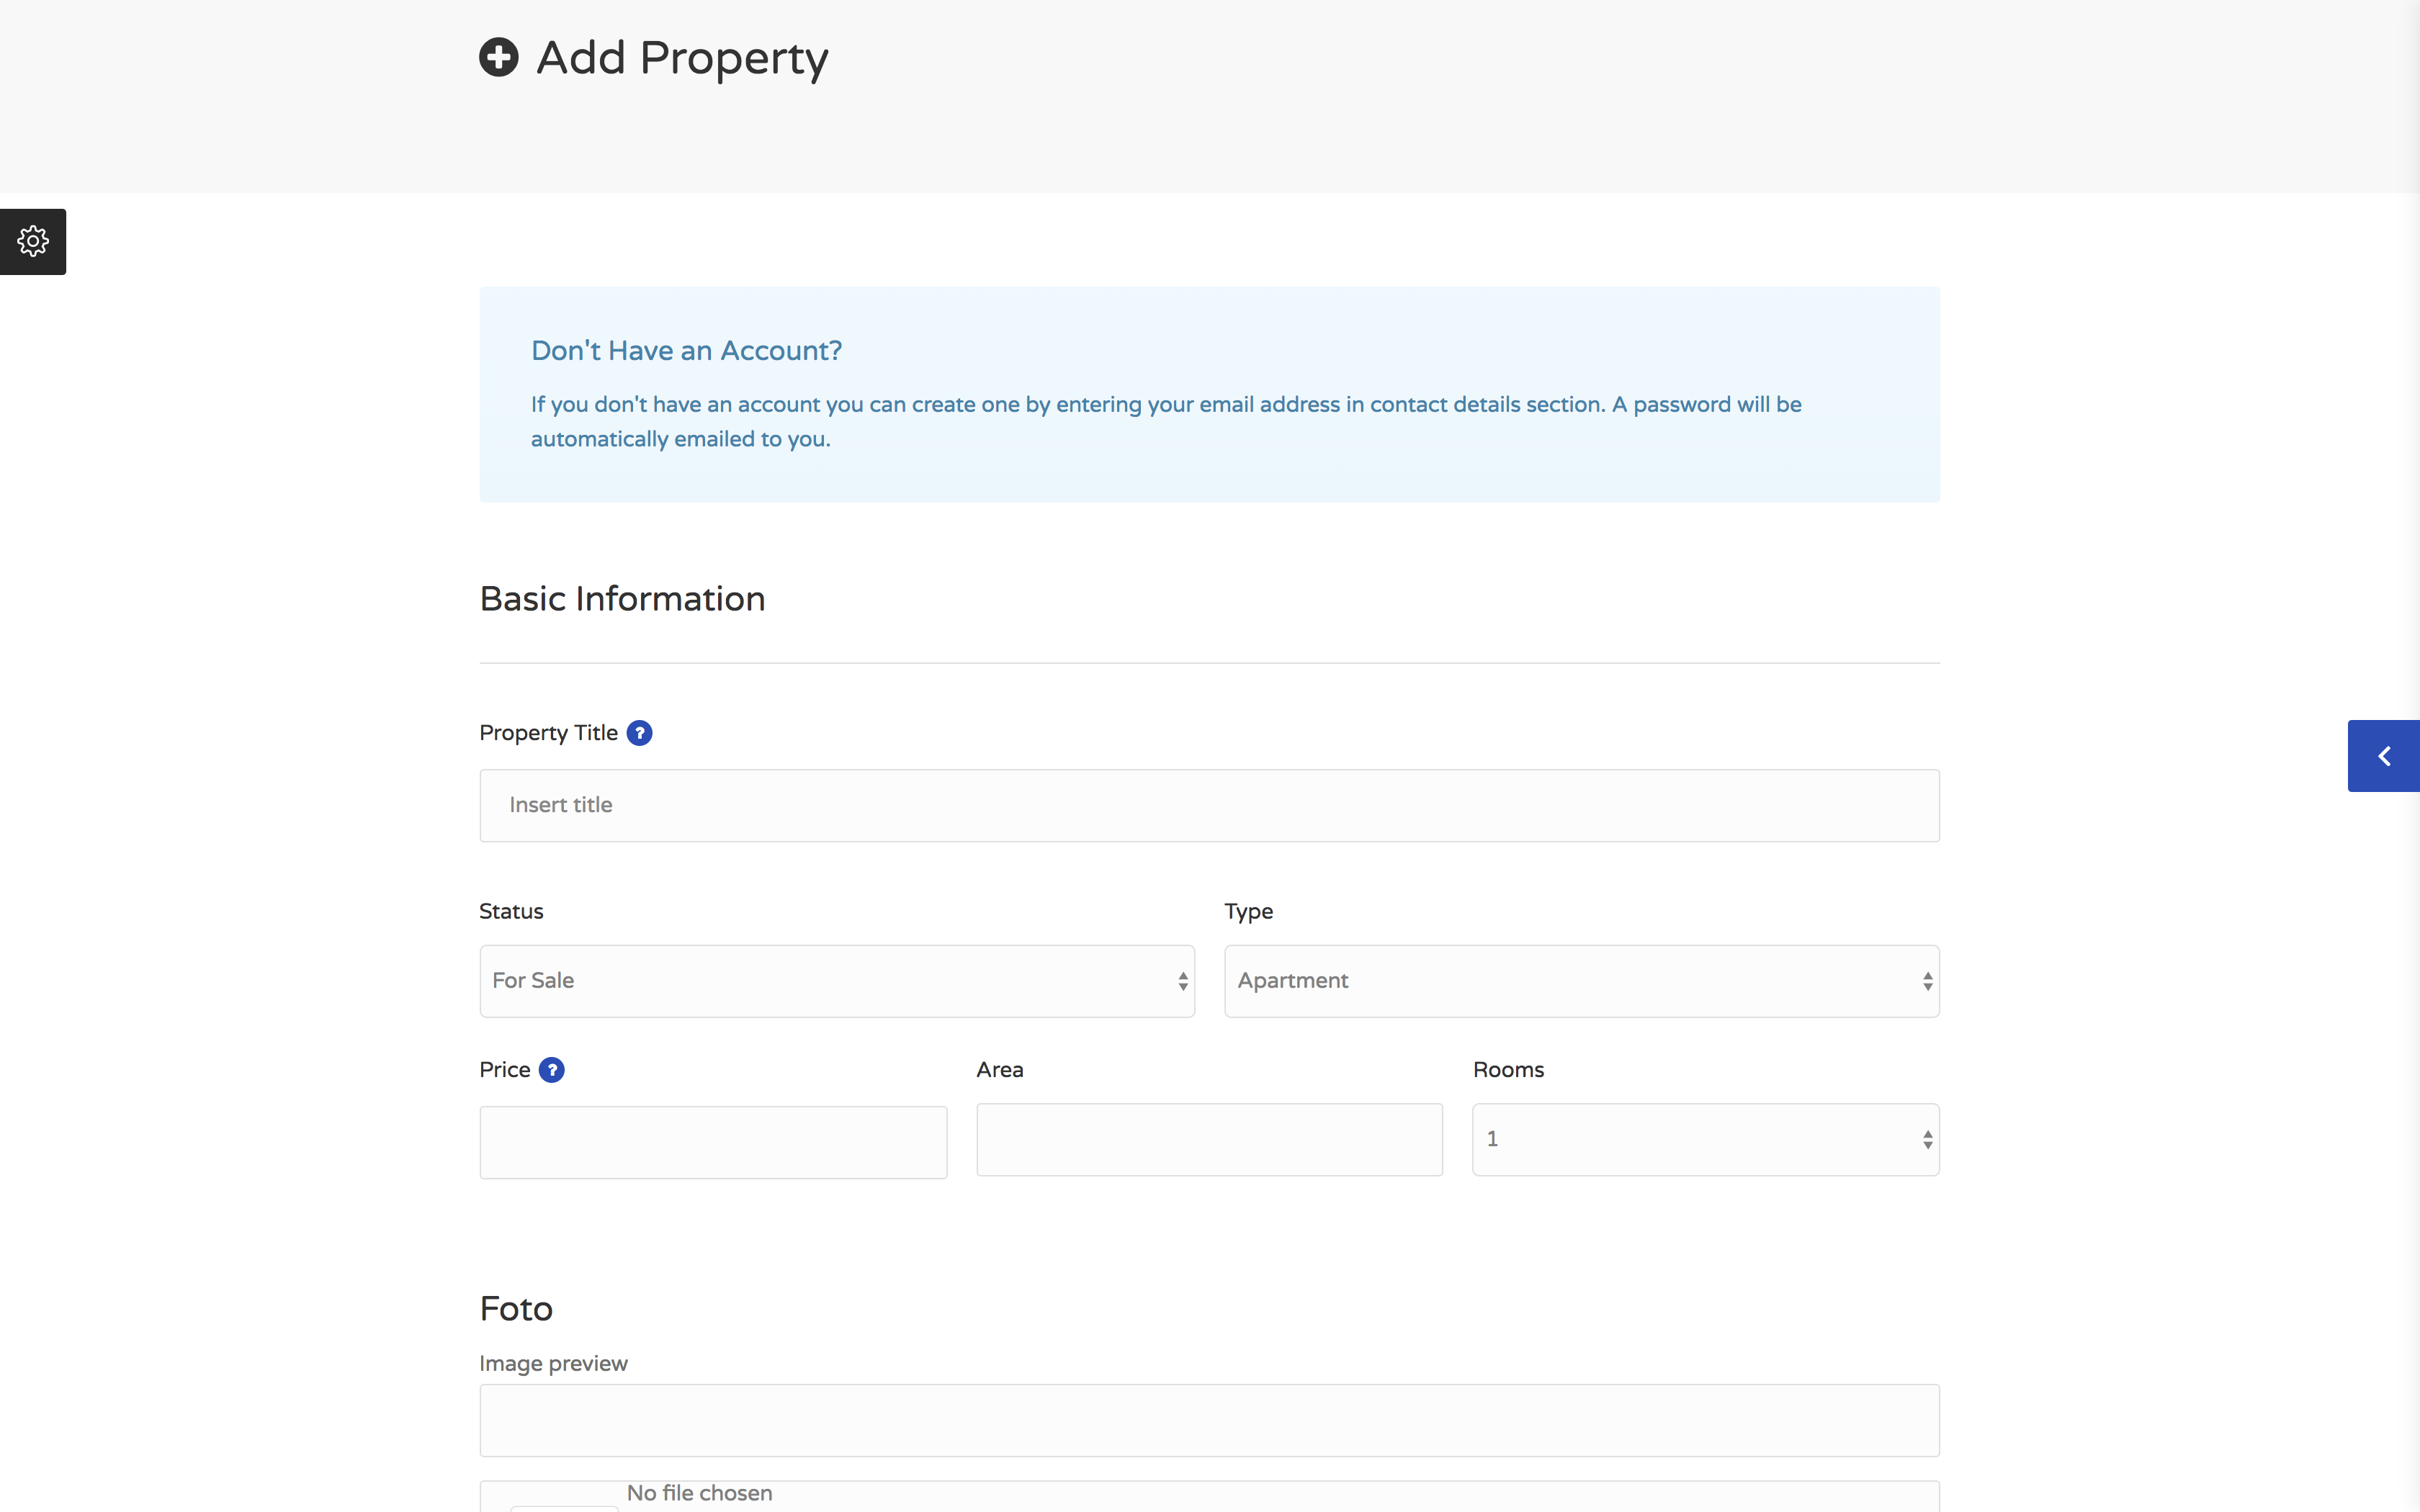
\includegraphics[width=0.75\textwidth]{img3.png}
\caption{}
\end{figure} 

\begin{figure}[H]
\centering
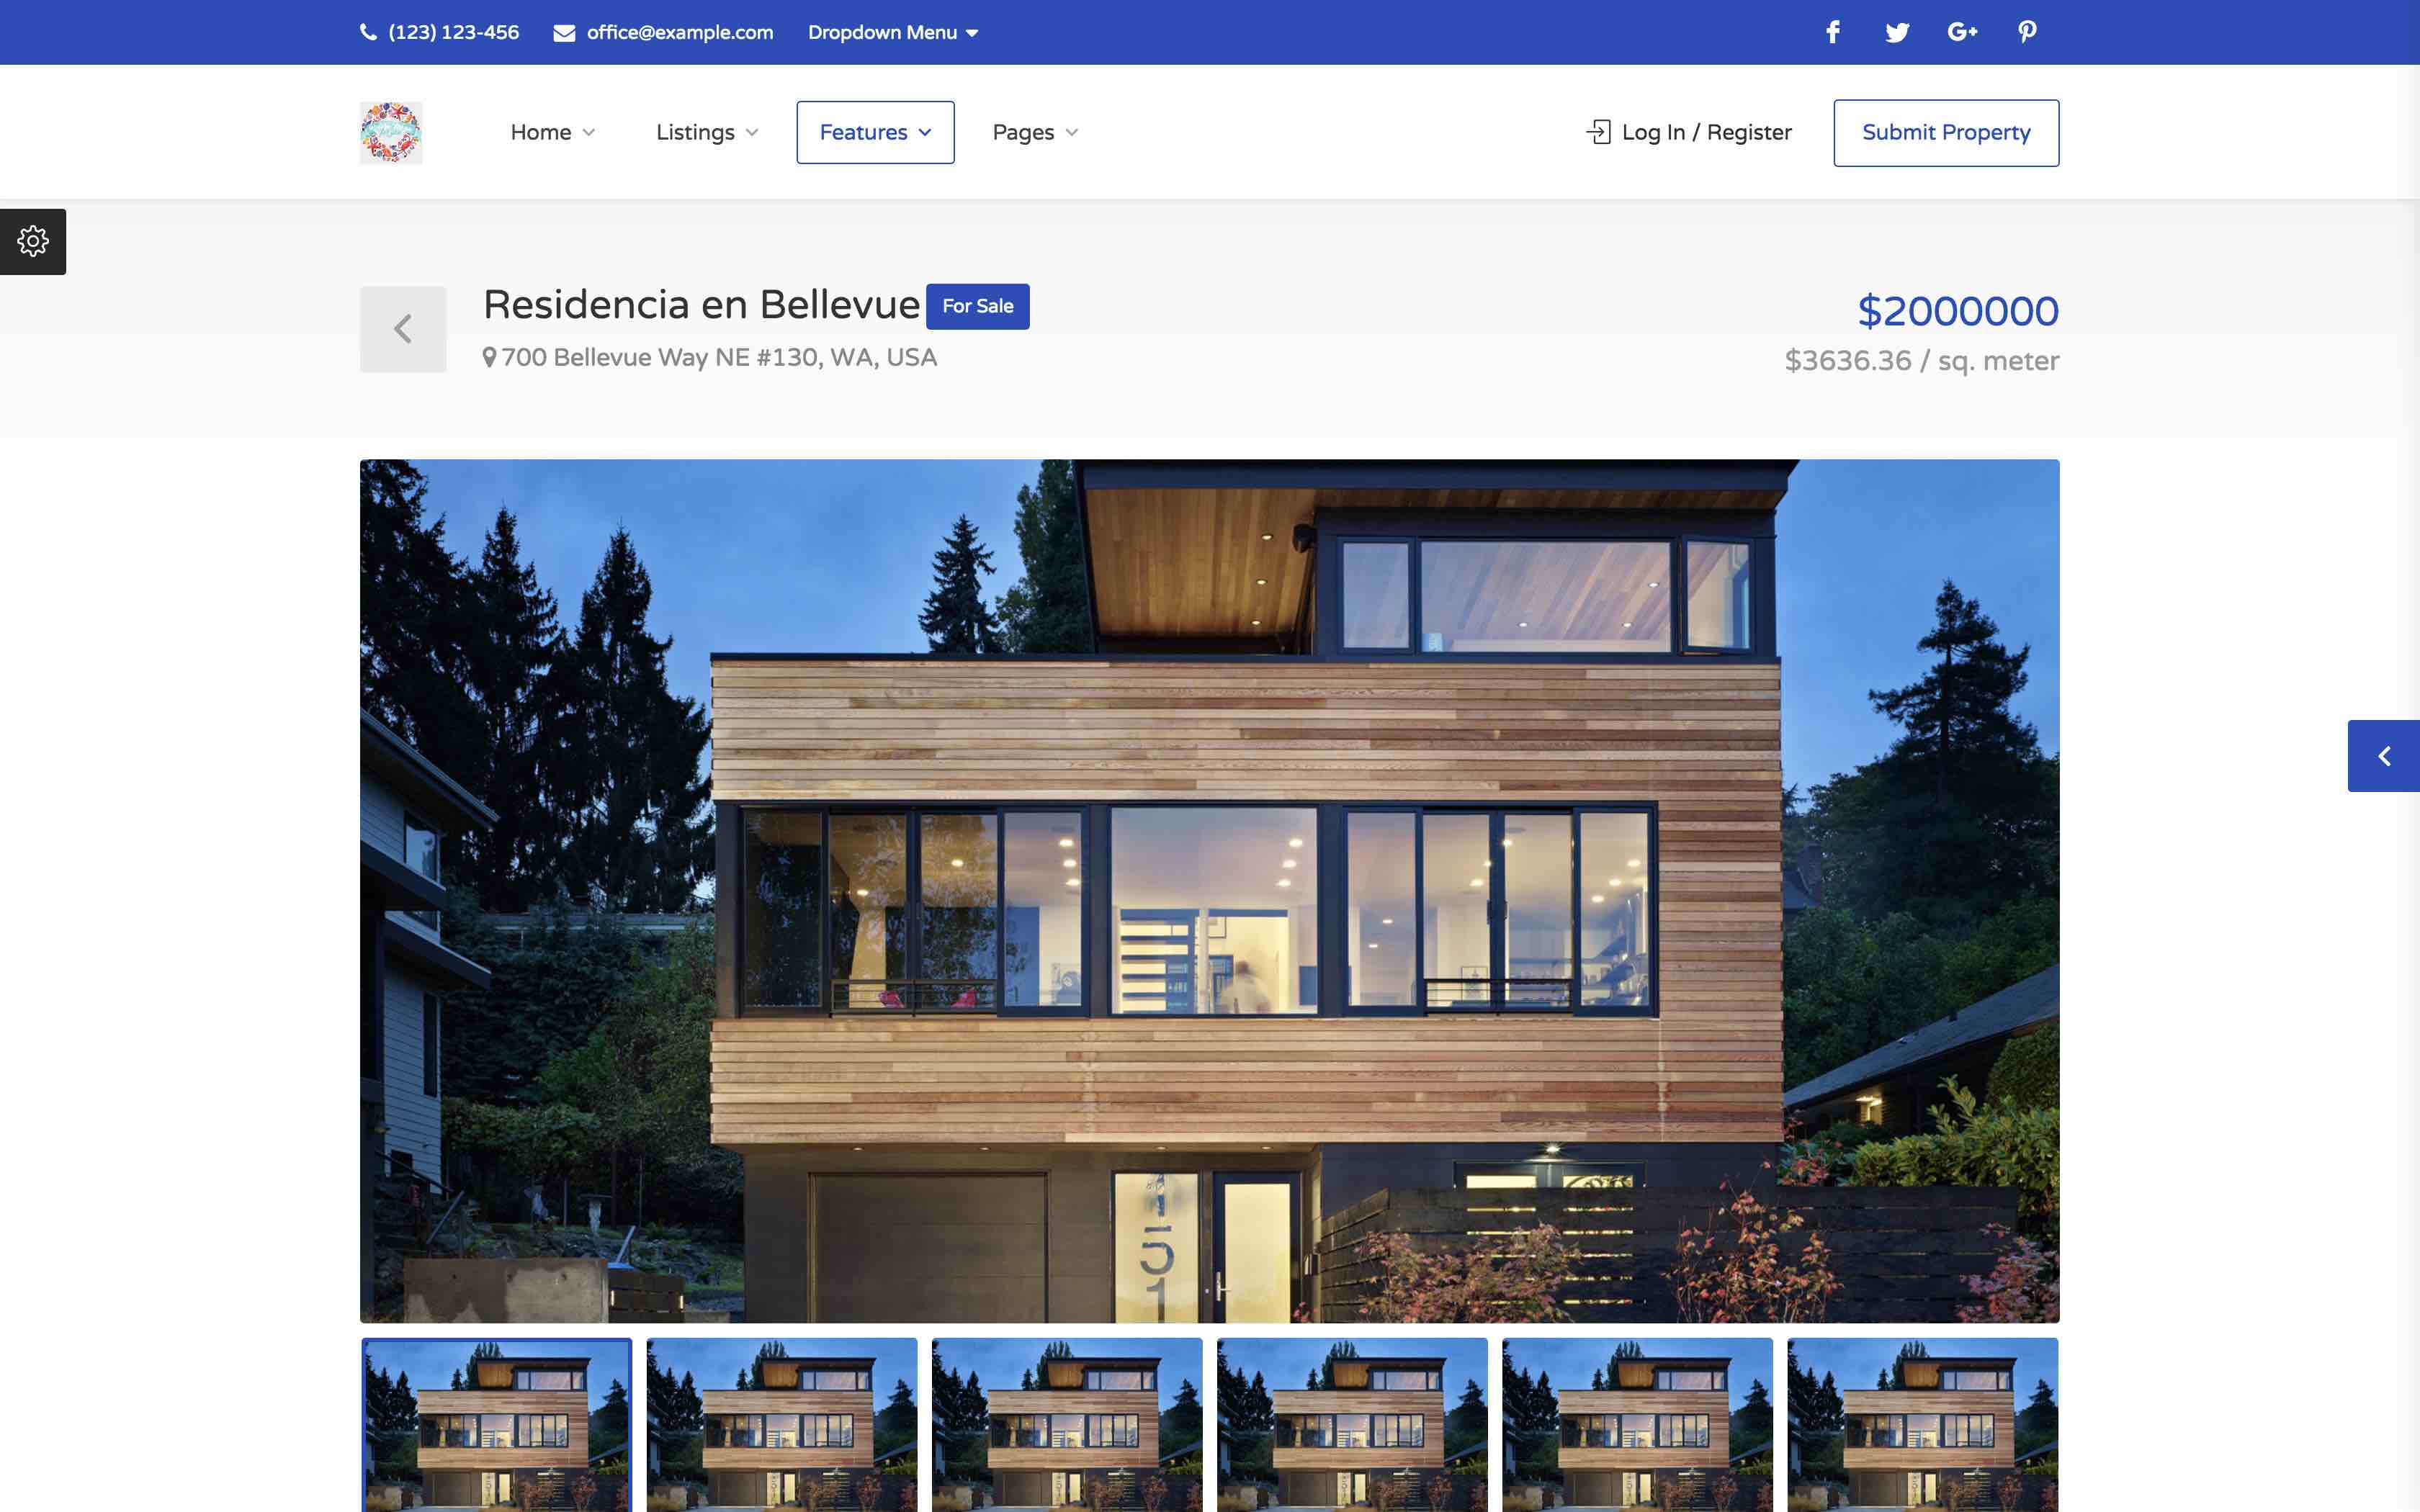
\includegraphics[width=0.75\textwidth]{img4.jpg}
\caption{}
\end{figure} 

\bibliographystyle{plain}
% \renewcommand{\bibliographyname}{Contenido}
\bibliography{biblist}

[1] Google. (n.d.). The Python NDB Client Library Overview  |  App Engine standard environment for Python  |  Google Cloud Platform. Consultado el 29 de noviembre de 2017 en https://cloud.google.com/appengine/docs/standard/python/ndb \linebreak

[2] Google. (n.d.). SDK de Google Cloud  |  Google Cloud Platform. Consultado el 29 de noviembre de 2017 en  https://cloud.google.com/sdk/?hl=es \linebreak

[3] Google. (n.d.). Datastore: base de datos NoSQL sin esquema  |  Google Cloud Platform. Consultado el 29 de noviembre de 2017 en https://cloud.google.com/datastore/?hl=es \linebreak


[4] Google. (n.d.). Architecture: Web Application on Google App Engine  |  Architectures  |  Google Cloud Platform. Consultado el 29 de noviembre de 2017 en  from https://cloud.google.com/solutions/architecture/webapp \linebreak

[5] Google. (n.d.). Cloud Endpoints: administración de APIs  |  Google Cloud Platform. Consultado el 29 de noviembre de 2017 en https://cloud.google.com/endpoints/?hl=es \linebreak

\end{document}